\subsection{Neural network used}

As used in~\cite{funker_large_2019} we will use a U-net, however we must adapt
it since we will only predict in 2D. Our first attempts at implementing the
U-net were not successful so we opted to used an already tried and tested
implementation, since we do not need to reimplement the wheel.\\
We used the implementation available at
\hyperlink{https://github.com/jvanvugt/pytorch-unet/}{github.com/jvanvugt/pytorch-unet/}.

\begin{figure}[!htbp]
	\centering
	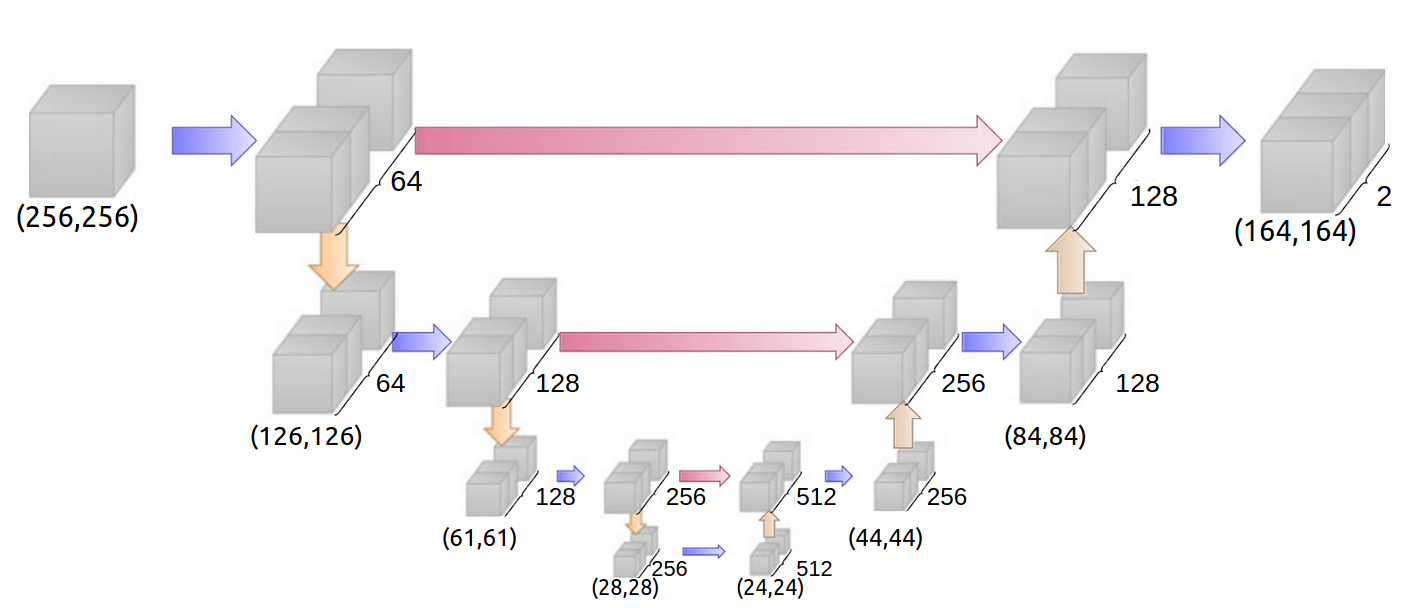
\includegraphics[width=1\linewidth]{./images/archi_unet.png}
	\caption{Architecture used for our experiments,
	from~\cite{funke_large_2019} with adjustments to numerical values}%
	\label{fig:archi_unet}
\end{figure}

We can see in figure~\ref{fig:archi_unet} the architecture that we used in
practice.\\
Here are the meaning of the various arrows :
\begin{itemize}
	\item Blue rightward arrows : two convolutionnal layrs, with kernel size
		$3\times3$, and ReLU activation after each convolution.
	\item Orange downward arrows : max pooling with size $2\times2$
	\item Brown upward arrows : bilinear upsampling of factor 2 folowed by a
		$1\times1$ convolutionnal layer to reduce the number of filters.
	\item Red rightward arrows : center crop and concatenation.
\end{itemize}
We will also note that we used batch normalization as it gave us more
consistent results in practice.\\
In~\cite{funke_large_2019} Kronecker matrix product is used for upsampling, we
opted to use bilinear upsampling as it gave us better results than transposed
convolutions and is more widely used, such as in~\cite{ronneberger_2015}.\\

The absence of padding in our convolutions is really useful as it allow us to
compute the loss over a smaller patch, speeding up the training quite
significatively.

\subsection{Use of a BPT to compute the loss}

Just like before, we used a Binary Partition Tree to help us compute our
loss.\\
Before, we used it to find the maximin edge by finding the lowest common
ancestor of our pixel pair.\\

However now we will use it as with Higra it gives us directly the area of
every nodes. Since every non-leaf node in the BPT corresponds to the addition
of an edge in our MST, we can easily obtain our areas needed to compute $w_n$
and $w_p$ in our loss function.\\

However here the hierarchical nature of the BPT is not really used, as a
modified Kruskal's algorithm could give us the same results, but here it was
the best tool for the task for which we had an optimized implementation.

\subsection{Inconsistent predictions along axes}
\begin{figure}[!htbp]
    \centering
    \begin{subfigure}[t]{0.40\textwidth}
        \centering
        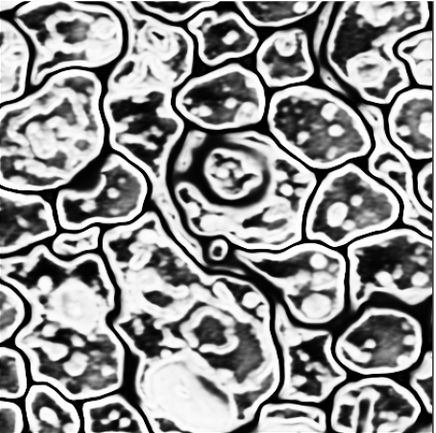
\includegraphics[height=0.9\textwidth]{./images/x_axis.png}
        \caption{Affinity along the X axis}
    \end{subfigure}%
    \begin{subfigure}[t]{0.40\textwidth}
        \centering
        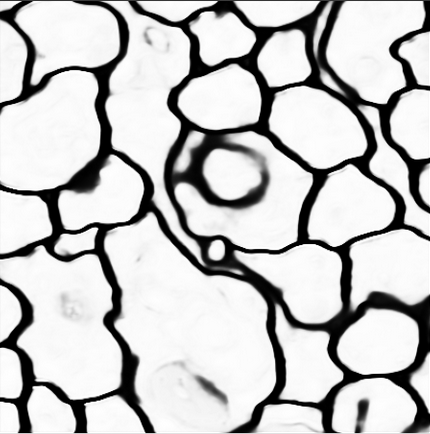
\includegraphics[height=0.9\textwidth]{./images/y_axis.png}
        \caption{Affinity along the Y axis}
    \end{subfigure}
	\caption{Example predicted affinities, notice the discrepancies between
	both.}
	\label{fig:affinity}
\end{figure}

As we can see in figure~\ref{fig:affinity} there are some important
discrepancies between our predictions, which we would not expect.\\
We can see that the two are almost the complementary of each other, with only
object borders in common. Ideally we eould want very similar results, are on
such a scale, the differences along an axis or the other should be small.

\begin{figure}[!htbp]
	\centering
	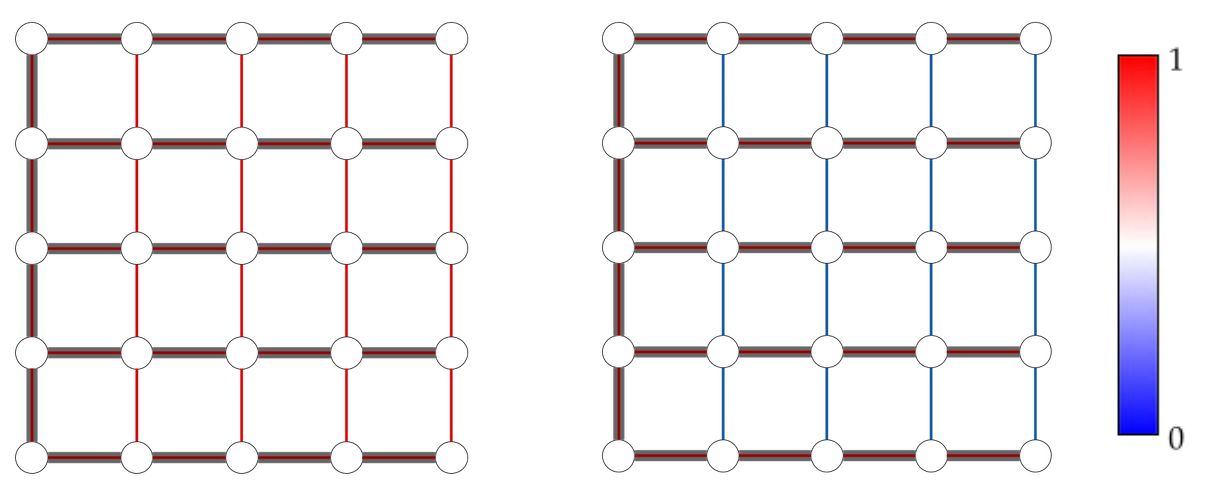
\includegraphics[width=0.8\linewidth]{./images/discrepancies_graph.png}
	\caption{Illustration of the discrepancies on a simpler graph. The
	groundtruth here would be to predit only red edges. In grey is drawn a
valid maximum spanning tree for both graph.}%
	\label{fig:discrepancies-graph}
\end{figure}

As we can see in figure~\ref{fig:discrepancies-graph} the scenario that we have
is represented by the graph on the right, where one axis has the value that we
would expect and the other does not except for its border.\\
Although the graphs are very different, they have the sane MST, and thus the
same MALIS loss, so both are perfectly valid and the neural network has no
incetive to choose one over the other. Sadly we would like the graph on the
right, as it could ease our post processing if the obtained graphs were more
similar to the truth, but the loss only forces the MSTs to be similar.\\

An explanation for this could be the way the MST is generated. Using Kruskal's
algorithm when multiple edges have the same value we need to make a choice, in
our case we pic kthe first edge with such value, but we could pick the last
one, or a random one for example. This could help to avoid such structures in
our graph, but this would need testing.\\
An other idea would be to use another loss that penalizes the general graph and
not just its MST, by comparing each edge to its groundtruth for example.
Combining both loss may lead to get the best of both worlds, but it would
require testing.

\subsection{Post processing}

We tried various different post processing, each with a different degree of
success, and we will present the most meaningful ones (in our opinion).

\subsubsection{Watershed}

At first we wanted to stay close to the post-processing proposed in the first paper.
Once we had predicted the two gradients, we merged them into one image by
attributing to each edge the average of the corresponding edges in the two
predicted images. Once this image was obtained, we did a simple threshold.\\
We then applied a watershed to obtain our final segmentation.\\

\begin{figure}[!htbp]
    \centering
    \begin{subfigure}[t]{0.31\textwidth}
        \centering
        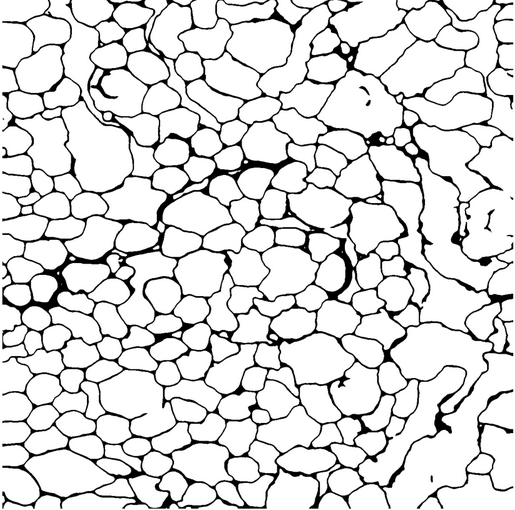
\includegraphics[height=0.9\textwidth]{./images/thresh_1.png}
		\caption{$\theta = 0.25$}
    \end{subfigure}%
    \begin{subfigure}[t]{0.31\textwidth}
        \centering
        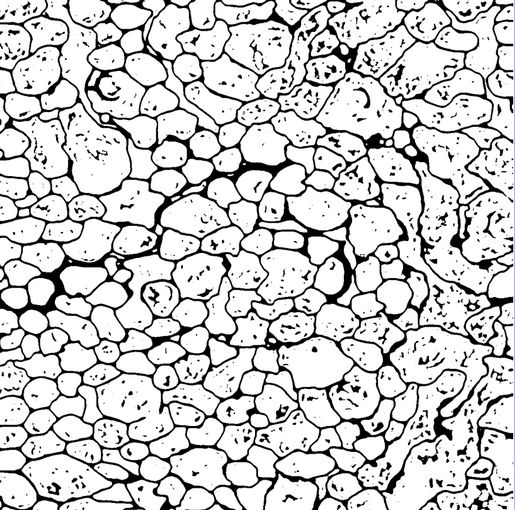
\includegraphics[height=0.9\textwidth]{./images/thresh_2.png}
        \caption{$\theta = 0.5$}
    \end{subfigure}%
    \begin{subfigure}[t]{0.31\textwidth}
        \centering
        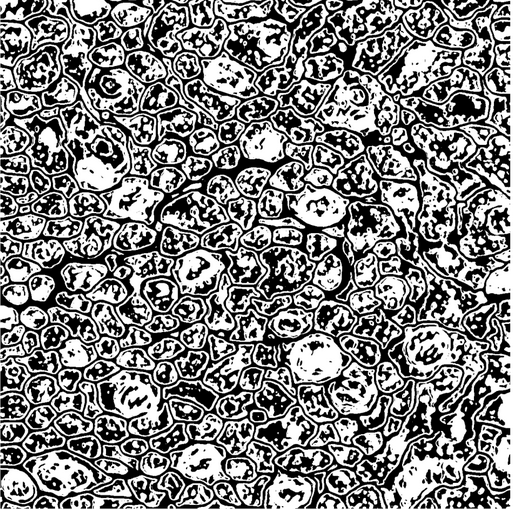
\includegraphics[height=0.9\textwidth]{./images/thresh_3.png}
        \caption{$\theta = 0.75$}
    \end{subfigure}
	\caption{Influence of the threshold parameter $\theta$}
	\label{fig:threshold}
\end{figure}

As we can see in figure~\ref{fig:threshold} we had to tweak the threshold
parameter in order to adjust the segmentation
level. With a too high $\theta$ value, there is too much data remaining in our
thresholded image. This could lead to over segmentation. On the contrary, with
a too low value, we risk seeing some segments merging. It is therefore
important to choose $\theta$ carefully in order to avoid these two cases which
drastically lower the Rand Index. In practice between 0.25 and 0.5 gave us very
similar results, both to the eye and using various metrics.\\

This technique is the one that gave us the best results. In addition to the
quality of the post-processing, it is also the fastest method: on a 2D image of
$1250\times1250$ from the CREMI dataset, it takes less than a second to get the result.
This is made possible because we use the implementation of an algorithm with
linear complexity from~\cite{cousty_watershed_2009} with Higra.\\

This method can also be couple with an agglomeration scheme afterwards, like
merging regions by area for example, but this did not give us interesting
results.

\subsubsection{Mumford-Shah functional}

We had a lot of trouble using this technique which proved to be very complex to
handle. After several experiments we only obtained segmentations that took the
cell nucleus into account, as in figure~\ref{fig:mumford-shah}.

\begin{figure}[!htbp]
	\centering
	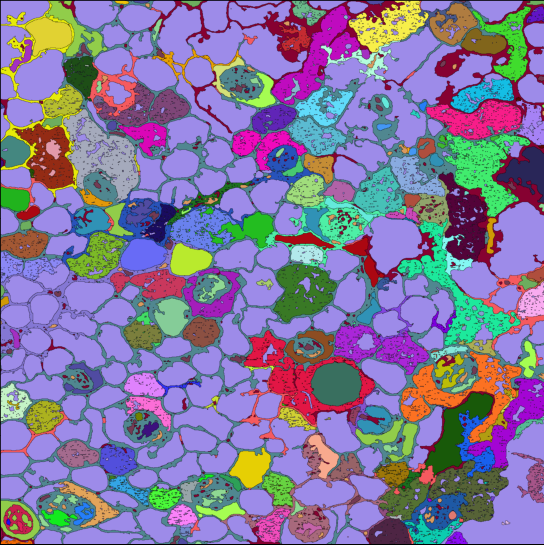
\includegraphics[width=0.3\linewidth]{./images/mumford_shah.png}
	\caption{Example of a result using Mumford-Shah for post processing}%
	\label{fig:mumford-shah}
\end{figure}

On top of that, the treatment is very long. For a 2D image of $1250\times1250$ from the
CREMI dataset,  it could take several minutes. Which is not sustainable knowing that
MALIS is made to work on 3D images.\\

We tried to reduce this computation time time by
using~\cite{perret_removing_2019}
as an inspiration, but without success. We would probably need more time to
better understand this technique and how to use it with Higra.


\subsubsection{Agglomeration in the region adjacency graph}

We also tried to implement the same processing that was used
in~\cite{funke_large_2019} but did not have the time to implement an optimised
version, as described in the paper.\\
We had to recompute the whole region adjacency graph at every step, which made
it very slow, especially when we started from an oversegmentation.\\

As such we chose not to use this method, but are confident that it would
improve our results, as it is quite a smart idea, that takes full advantage of
the affinities.




\subsection{An improved way to generate edge weights}

One of the issues that we had before was that when computing the edge weights we lost the gradient
information, which forced us to go back to our neural network's output, which was costly.
However a change in Higra's function to compute edge weights forced us to adapt and find a better
method, which will describe here.\\

\begin{figure}[!htbp]
	\centering
	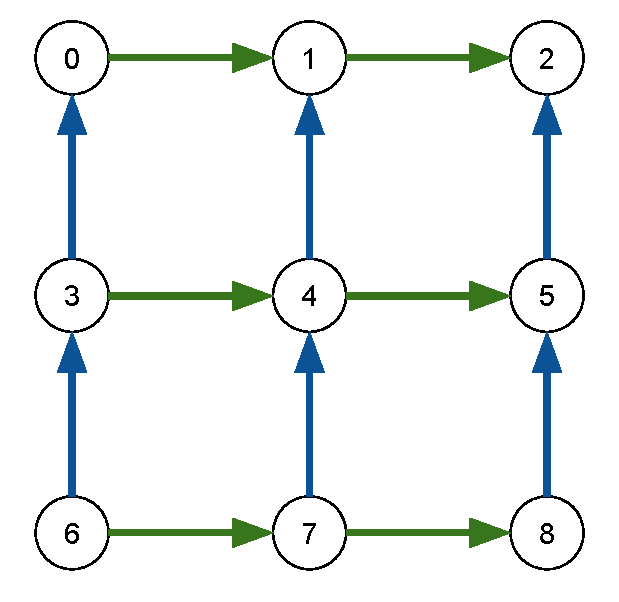
\includegraphics[width=0.4\linewidth]{./images/graph.pdf}
	\caption{Construction of a 4 connected graph in 2d. Green edges represent x
	edges and blue edges represent y edges}%
	\label{fig:graph}
\end{figure}

As we can see in figure~\ref{fig:graph} there is a straightworward way to
relate our edges and their counterpart in the neural network output.\\

The only constraint that we have for the construction of the edge weights is to
use operations supported by our deep learning library of choice. For PyTorch, this
includes if statements, min, max, all array indexing methods etc.

\subsubsection{Weighting edges with Higra}

Once we have our edge weighting function, we can directly use Higra to get our
edge weights.
\begin{lstlisting}[language=Python]
import higra as hg

# Both variables were obtained from our NN
x_edges = ...
y_edges = ...

#Building our graph
graph = hg.get_4_adjacency_graph(x_edges.shape)

#Getting our edges and computing their weights
src, dst = graph.edge_list()
weights = weight_function(src,dst,x_edges,y_edges)
\end{lstlisting}

This will work in the general case, but in the case of a 4 connected graph and
with the way our neural network generates edge weights we can optimise this.
Indeed the edge list is obtained in a structured and deterministic way which
we will now decsribe.


\subsubsection{Higra's edge weights structure}

\begin{figure}[!htbp]
	\centering
	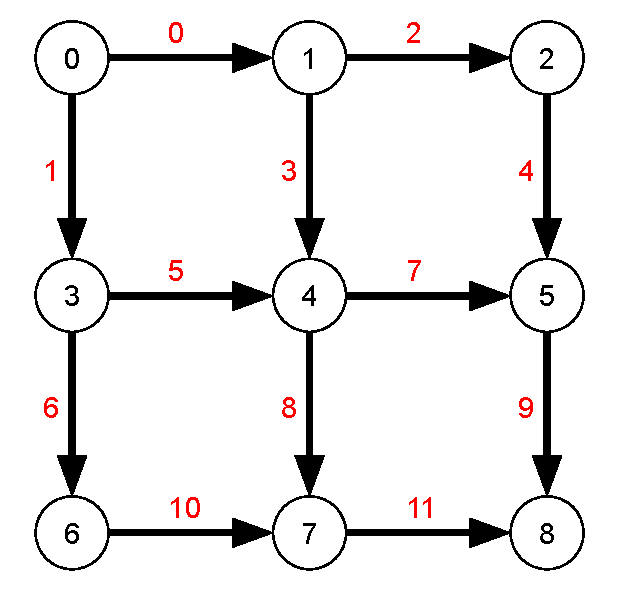
\includegraphics[width=0.4\linewidth]{./images/graph-order.pdf}
	\caption{Oder of edges obtained using Higras's \textit{edge\_list}
	function.}%
	\label{fig:graph_order}
\end{figure}

As we can see in figure~\ref{fig:graph_order} edges are always obtained in the
same fashion, which will allow us to develop a function that bypasses the call
to \textit{edge\_list} since they will always be in the same order.\\
The constraint are thus that we need to respect this order in our function, and
we need to be careful about code maintenance and unit tests, as a change of the
way the edges are obtained would break our method.\\
To alleviate those risks, the best method is to create tests comparing our
method and the official method, which is guaranteed to work.


\subsubsection{Our method to generate edge weights}

\begin{figure}[!htbp]
\centering
\begin{minipage}[c]{0.2\textwidth}
\centering
\[
	\text{x\_edges}=
  \begin{bmatrix}
	  1 & 2 & 3 \\
	  4 & 5 & 6 \\
	  7 & 8 & 9 \\
  \end{bmatrix}
\]
\end{minipage}\hfill
\begin{minipage}[c]{0.2\textwidth}
\centering
\[
	\text{y\_edges}=
  \begin{bmatrix}
	  -1 & -2 & -3 \\
	  -4 & -5 & -6 \\
	  -7 & -8 & -9 \\
  \end{bmatrix}
\]

\end{minipage}\hfill
\begin{minipage}[c]{0.45\textwidth}
\centering
    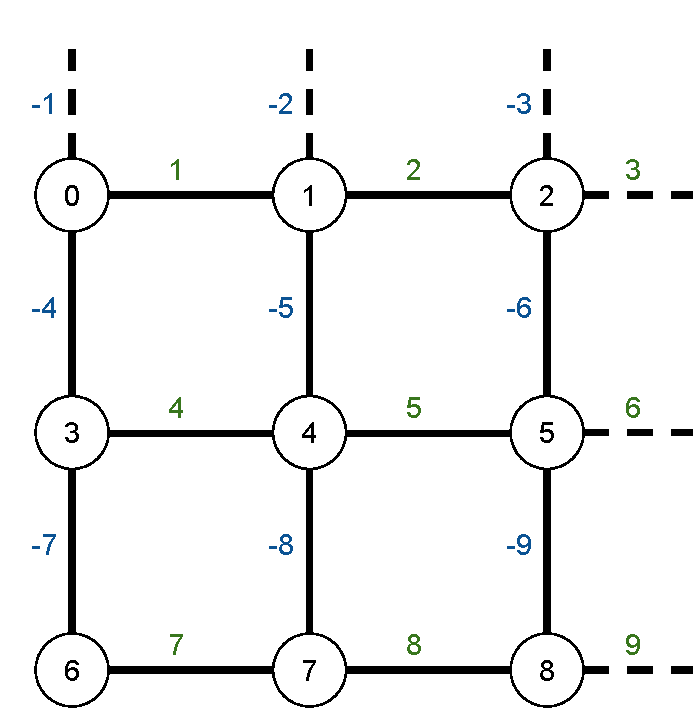
\includegraphics[width=\textwidth]{./images/edge_weights_predicted.pdf}
\end{minipage}

    \caption{Example of desired results from our x and y edges predicted by our
	neural network. Notice that some edges are not contained in the image. Even
though they are present in our NN output we will remove them from the graph}
    \label{fig:ew_predicted}
\end{figure}

As we can see in figure~\ref{fig:ew_predicted}, we get edge matrices the same
size as our image, but if our image is of dimension $n\times m$ we only need a
matrix of size $n\times (m-1)$ for our edges in the y direction and of size
$(n-1)\times m$ for our edge in the x direction.\\
The choice to have those irrelevant edge weights is simply for ease of use, and
to ease the design of the NN output.\\

As we can also see, our edge weights are simply a
kind of entanglement of our x and y edges. This leads us to the following code
to generate of edge weights which doesn't rely on Higra's function :
\begin{lstlisting}[language=Python]
import higra as hg
import torch

# Both variables were obtained from our NN
x_edges = ...
y_edges = ...

# Getting our edge weights

height,width=x.shape
# Removing the out of graph edges
x_u  = x_edges[:-1].T[:-1]
y_u = y_edges[1:].T

edge_weights = torch.from_numpy(np.empty((2*width-1,height-1),dtype=np.float64))
edge_weights = edge_weights.type(torch.FloatTensor).to(device)

# Creating the entanglement
edge_weights[0:-1:2,:] = x_u
edge_weights[1::2,:] = y_u[:-1]
edge_weights[-1] = y_u[-1]

#Adding back missing x edges
edge_weights= torch.cat((edge_weights.T.flatten(),x_edges[-1,:-1]))
\end{lstlisting}

This example here is using PyTorch, but an analogous version for numpy can be
made by replacing function names.\\

Using this code we are able to generate edge weights very fast and we are sure
that our edge weights will contain the gradient history, which is what we
wanted.

\subsubsection{Backpropagation}

Once we have our edge weights as an array, for any processing that we will have
to do, we can refer to the edge weights which are guaranteed to contain the
gradient information. This is easier that going back to the NN output, where we
would have to reverse the code used to get our edge weights to find their
position in the output.\\

This process of going back to our neural network was very costly and caused a
very important bottleneck in our code, which this solution alleviated
instantly. We had a backward pass that was taking 100 times as long as our
forward pass, which should not be the case, we expected it to be 2 or 3 times
as ong at most.
